% !TeX spellcheck = it_IT

\documentclass[]{beamer}

\usepackage[utf8]{inputenc}
\usepackage[italian]{babel}
\usepackage{multicol}
\usetheme{metropolis}

\usepackage{tikz}
\usetikzlibrary{shapes,arrows,positioning}

\tikzstyle{startstop} = [ellipse, draw, fill=bg, text=structure, text width=3em, text badly centered, inner sep=0pt]
\tikzstyle{block} = [rectangle, draw, fill=bg, text=structure, text width=5em, text centered]
\tikzstyle{decision} = [diamond, aspect=3, draw, fill=bg, text=structure, text width=3em, text badly centered, inner sep=0pt]
\tikzstyle{input} = [trapezium, draw, fill=bg, text=structure, text width=5em, text centered, trapezium right angle=120]
\tikzstyle{output} = [trapezium, draw, fill=bg, text=structure, text width=5em, text centered, trapezium right angle=120]

\tikzstyle{line} = [draw, -latex']


\title{Informatica B - Esercitazione 1}
\subtitle{Algoritmi e schemi a blocchi}

\author{Stefano Cereda\\
		stefano.cereda@polimi.it
	}
\date{25/09/2018}
\institute[PoliMi]{\vspace{0.5cm}\centering Politecnico di Milano \\ \vspace{0.2cm}
	
\includegraphics[width=0.2\linewidth]{../logopolimi}}

\setbeamercovered{invisible}

\makeindex

\begin{document}
\begin{frame}
	\maketitle
\end{frame}

\begin{frame}
\frametitle{Approccio ai problemi}
\begin{enumerate}
	\item Comprensione problema
	\item Divide et impera
	\item Raffinamenti successivi
	\item Scrittura soluzione
	\item Test della soluzione
\end{enumerate}
\end{frame}

\begin{frame}
	\frametitle{Schemi a blocchi - Costrutti}
	\begin{tikzpicture}[node distance = 1cm, auto]
		\node [startstop] (start) {Inizio};
		\node [input, below = of start] (in) {Leggi};
		\node [inner sep=0pt, right = 5.5 of in] (imgIN) {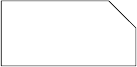
\includegraphics[width=.15\textwidth]{blocco_in}};
		\node [block, below = of in] (increment) {Fai};
		\node [decision, below = of increment] (decision) {?};
		\node [output, below left = of decision] (outpos) {Scrivi};
		\node [output, below right = of decision] (outneg) {Scrivi};
		\node [inner sep=0pt, below = 3.5 of imgIN] (imgOUT) {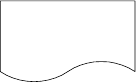
\includegraphics[width=.15\textwidth]{blocco_out}};
		\node [startstop, below = 1.5 of decision] (stop) {Fine};
		
		\path [line] (start) -- (in);
		\path [line] (in) -- (increment);
		\path [line] (increment) -- (decision);
		\path [line] (decision) -| node [near end] {vero} (outpos);
		\path [line] (decision) -| node [near end] {falso} (outneg);
		\path [line] (outpos) -- (stop);
		\path [line] (outneg) -- (stop);
		
		\node [right = 1.5 of start] {Blocco di inizio};
		\node [right = 1.5 of in] {Blocco di ingresso dati};
		\node [right = 1.5 of increment] {Blocco di esecuzione};
		\node [right = 1.5 of decision] {Blocco di condizione};
		\node [right = .5 of outneg] {Blocco di uscita dati};
		\node [right = 1.5 of stop] {Blocco di fine};
		\end{tikzpicture}

\end{frame}

\begin{frame}
\centering
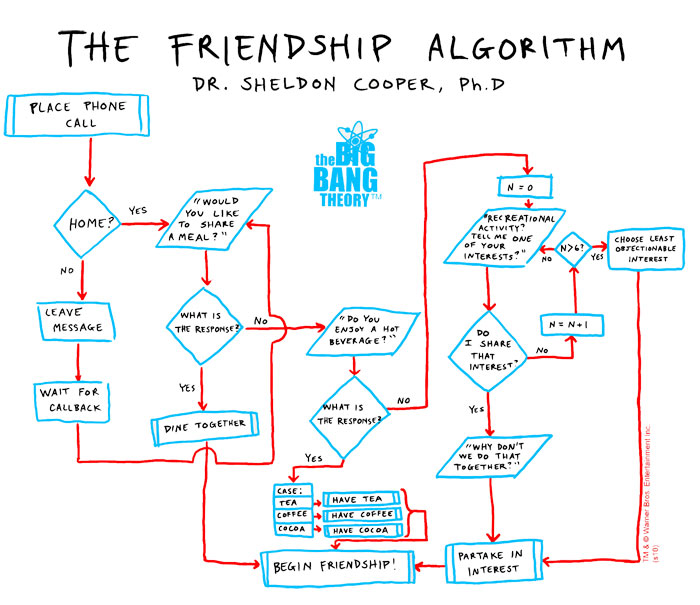
\includegraphics[height=\textheight]{block_sheldon.png}
\end{frame}

%ESEMPIO 1
\begin{frame}
	\frametitle{Esempio 1 - Ordinamento coppie di numeri}
	Scrivere un programma che, ricevuti in input due numeri \emph{a} e \emph{b}, li stampi in ordine dal più piccolo al più grande.
\end{frame}

\begin{frame}
	\frametitle{Esempio 1 - Soluzione con schema a blocchi}
	\centering
		\begin{tikzpicture}[auto]
	\node [startstop] (start) {Inizio};
	\node [input, below = of start] (input) {Leggi a,b};
	\node [decision, below = of input] (decision) {a $<$ b};
	\node [output, below left = of decision] (outab) {Stampa a,b};
	\node [output, below right = of decision] (outba) {Stampa b,a};
	\node [startstop, below = 2.5 of decision] (stop) {Fine};
	
	\path [line] (start) -- (in);
	\path [line] (in) -- (decision);
	\path [line] (decision) -| node [near start] {vero} (outab);
	\path [line] (decision) -| node [near start] {falso} (outba);
	\path [line] (outab) -- (stop);
	\path [line] (outba) -- (stop);
	\end{tikzpicture}

\end{frame}

\begin{frame}
	\frametitle{Esempio 1 - Soluzione in pseudocodice}
	\begin{enumerate}
		\item Leggo due numeri \emph{a} e \emph{b}
		\item Se \emph{a} è minore di \emph{b}:
		\begin{enumerate}
			\item Stampa su schermo \emph{a} e \emph{b}
		\end{enumerate}
		\item Altrimenti:
		\begin{enumerate}
			\item Stampa su schermo \emph{b} e \emph{a}
		\end{enumerate}
		\item Fine
	\end{enumerate}
\end{frame}

%ESERCIZIO 1
\begin{frame}
	\frametitle{Esercizio 1 - Calcolo della divisione e del resto}
	Scrivere un programma che, ricevuti in ingresso due numeri \emph{a} e \emph{b}, stampi il risultato della divisione \emph{a/b} ed il relativo resto.
	
	Se l'operazione non è possibile, il programma termina senza stampare alcun messaggio.
	
	Utilizzare l'operatore modulo \% per calcolare il resto della divisione.
\end{frame}

\begin{frame}
	\frametitle{Esercizio 1 - Soluzione con schema a blocchi}
		\centering
	\begin{tikzpicture}[node distance = .5cm, auto]
	\node [startstop] (start) {Inizio};
	\node [input, below = of start] (input) {Leggi a,b};
	\node [decision, below = of input] (decision) {b $\neq$ 0};
	\node [block, below left = of decision] (div) {div = a/b};
	\node [block, below = of div, text width = 7 em] (mod) {mod = a\%b};
	\node [output, below = of mod] (out) {Stampa div,mod};
	\node [startstop, below = 4 of decision] (stop) {Fine};
	
	\path [line] (start) -- (input);
	\path [line] (input) -- (decision);
	\path [line] (decision) -| (div) node [near start] {true};
	\path [line] (decision) -- +(2,0) node[near start] {false} |- (stop);
	\path [line] (div) -- (mod);
	\path [line] (mod) -- (out);
	\path [line] (out) |- (stop);
	\end{tikzpicture}
\end{frame}

\begin{frame}
\frametitle{Esercizio 1 - Soluzione in pseudocodice}
\begin{enumerate}
	\item Leggo due numeri \emph{a} e \emph{b}
	\item Se \emph{b} è uguale a zero termino
	\item Assegno a \emph{div} il risultato della divisione intera tra \emph{a} e \emph{b}
	\item Assegno a \emph{mod} il resto della divisione intera tra \emph{a} e \emph{b}
	\item Stampo su schermo \emph{div} e \emph{mod}
	\item Fine
\end{enumerate}
\end{frame}

\iffalse
\begin{frame}
\frametitle{Esercizio 2 - Ordinamento}
Scrivere un programma che, ricevuti in ingresso tre numeri \emph{a}, \emph{b} e \emph{c}, li stampi in ordine decrescente.

TODO: ma qui non conviene fare un esempio di conversione binaria?
\end{frame}

\begin{frame}
\frametitle{Esercizio 2 - Soluzione con schema a blocchi}
\centering
\makebox[\textwidth]{\resizebox{1.1\linewidth}{!}{
\begin{tikzpicture}[auto]
	\node [startstop] (start) {Inizio};
	\node [input, below = .5 of start] (input) {a,b,c};
	\node [decision, below = .5 of input] (decision) {a $\geq$ b};
	
	\node [decision, below left = of decision] (decision1) {a $\geq$ c};
	\node [decision, below right = of decision] (decision2) {a $\geq$ c};
	
	\node [decision, below left = of decision1] (decision11) {b $\geq$ c};
	\node [decision, below right = of decision2] (decision22) {b $\geq$ c};
	
	\node [output, below left = of decision11] (outabc) {a,b,c};
	\node [output, right = .4 of outabc] (outacb) {a,c,b};
	\node [output, right = .4 of outacb] (outcab) {c,a,b};
	
	\node [output, below right = of decision22] (outcba) {c,b,a};
	\node [output, left = .4 of outcba] (outbca) {b,c,a};
	\node [output, left = .4 of outbca] (outbac) {b,a,c};
	
	\node [startstop, below = 5.5 of decision] (stop) {Fine};
	
	\path [line] (start) -- (input);
	\path [line] (input) -- (decision);
	\path [line] (decision) -- (decision1) node [near start, left] {true};
	\path [line] (decision) -- (decision2) node [near start] {false};
	
	\path [line] (decision1) -- (decision11) node [near start, left] {true};
	\path [line] (decision1) -- (outcab) node [near start] {false};
	
	\path [line] (decision11) -- (outabc) node [near start, left] {true};
	\path [line] (decision11) -- (outacb) node [near start] {false};
	
	\path [line] (decision2) -- (decision22) node [near start] {false};
	\path [line] (decision2) -- (outbac) node [near start, left] {true};
	
	\path [line] (decision22) -- (outcba) node [near start] {false};
	\path [line] (decision22) -- (outbca) node [near start, left] {true};
	
	\path [line] (outabc) -- (stop);
	\path [line] (outacb) -- (stop);
	\path [line] (outcab) -- (stop);
	\path [line] (outbac) -- (stop);
	\path [line] (outbca) -- (stop);
	\path [line] (outcba) -- (stop);
	
\end{tikzpicture}
}}
\end{frame}


\begin{frame}
\frametitle{Esercizio 2 - Soluzione in pseudocodice}
\begin{multicols}{2}
\begin{enumerate}
	\item Leggi \emph{a}, \emph{b} e \emph{c}
	\item Se $a \geq b$ vai a 3, altrimenti vai a 11
	
	\item Se $a \geq c$ vai a 4, altrimenti vai a 9
	\item Se $b \geq c$ vai a 5, altrimenti vai a 7
	\item Stampa \emph{a,b,c}
	\item Vai a 19
	\item Stampa \emph{a,c,b}
	\item Vai a 19
	\item Stampa \emph{c,a,b}
	\item Vai a 19
	
	\item Se $a \geq c$ vai a 13, altrimenti vai a 12
	\item Se $b \geq c$ vai a 15, altrimenti vai a 17
	\item Stampa \emph{b,a,c}
	\item Vai a 19
	\item Stampa \emph{b,c,a}
	\item Vai a 19
	\item Stampa \emph{c,b,a}
	\item Vai a 19
	
	\item Fine.
\end{enumerate}
\end{multicols}
\end{frame}

\fi

\begin{frame}
\frametitle{Esercizio 2 - Conversione in binario}
\alert{Da fare dopo aver visto il binario.}

Scrivere un programma che, ricevuto in ingresso un numero positivo \emph{n}, lo stampi in binario. Si utilizzi il metodo delle divisioni ripetute.

Per semplificare, si stampi separatamente ogni cifra del resto. Si stampi inoltre il risultato in ordine inverso.
\end{frame}

\begin{frame}
\frametitle{Esercizio 2 - Soluzione con schema a blocchi}
\centering
\begin{tikzpicture}[node distance = 1cm, auto]
\node [startstop] (start) {Inizio};
\node [input, below = of start] (input) {Leggi n};
\node [decision, below = of input] (while) {n $>$ 0};

\node [output, below right = of while] (out) {Stampa n\%2};
\node [block, below = of out] (divide) {n = n/2};

\node [startstop, below = 3.5 of while] (stop) {Fine};

\path [line] (start) -- (input);
\path [line] (input) -- (while);
\path [line] (while) -| (out) node[near start] {true};
\path [line] (out) -- (divide);
\path [line] (divide) -| (while);
\path [line] (while) -- +(-2,0) node[near start] {false} |- (stop);
\end{tikzpicture}
\end{frame}

\begin{frame}
\frametitle{Esercizio 2 - Soluzione in pseudocodice}
\begin{enumerate}
	\item Leggi \emph{n}
	\item Ripeti finché n è maggiore di 0:
	\begin{enumerate}
		\item Stampa il resto della divisione n/2
		\item Assegna ad \emph{n} la parte intera della divisione n/2
	\end{enumerate}
	\item Fine
\end{enumerate}
\end{frame}

\begin{frame}
\frametitle{Esercizio 3 - Calcolo del fattoriale}
Scrivere un programma che, ricevuto in ingresso un numero \emph{n}, ne calcoli e visualizzi il fattoriale.

Si assuma che l'utente non inserisca mai numeri minori di 1.

Si ricorda che il fattoriale di \emph{n} è definito come il prodotto di tutti i numeri fra \emph{n} ed 1: $n! = \prod_{i=1}^{n}i = 1 \cdot 2 \dots (n-1) \cdot n$
\end{frame}

\begin{frame}
\frametitle{Esercizio 3 - Soluzione con schema a blocchi}
		\centering
\begin{tikzpicture}[node distance = .5cm, auto]
\node [startstop] (start) {Inizio};
\node [input, below = of start] (input) {Leggi n};
\node [block, below = of input] (setI) {i = 1};
\node [block, below = of setI] (setRis) {ris = 1};
\node [decision, below = of setRis] (while) {i $<$ n};

\node [block, below left = 1 of while] (incI) {i = i + 1};
\node [block, below = of incI] (prod) {ris = ris $\cdot$ i};

\node [output, below right = 1 of while] (out) {Stampa ris};
\node [startstop, below = 1 of out] (stop) {Fine};

\path [line] (start) -- (input);
\path [line] (input) -- (setI);
\path [line] (setI) -- (setRis);
\path [line] (setRis) -- (while);
\path [line] (while) -- +(-2,0) node [near start] {true} -| (incI);
\path [line] (incI) -- (prod);
\path [line] (prod) -- +(2,0) -| (while);
\path [line] (while) -| (out) node[near start] {false};
\path [line] (out) -- (stop);
\end{tikzpicture}
\end{frame}

\begin{frame}
\frametitle{Esercizio 3 - Soluzione in pseudocodice}
\begin{enumerate}
	\item Leggi \emph{n}
	\item Assegna 1 alla variabile \emph{i}
	\item Assegna 1 alla variabile \emph{ris}
	\item Ripeti finché $i < n$:
	\begin{enumerate}
		\item Incrementa \emph{i} di 1
		\item Assegna a \emph{ris} il risultato di $ris \cdot i$
	\end{enumerate}
	\item Stampa il valore di \emph{ris}
	\item Fine
\end{enumerate}
\end{frame}

\begin{frame}
\frametitle{Esercizio 4 - Calcolo del minimo comune multiplo}
Scrivere un programma che, ricevuti in ingresso due numeri \emph{a} e \emph{b}, ne calcoli e visualizzi il minimo comune multiplo.

Si assuma che \emph{a} e \emph{b} siano sempre positivi.

Si ricorda che il minimo comune multiplo è definito come il più piccolo intero positivo multiplo sia di \emph{a} che di \emph{b}.
\end{frame}

\begin{frame}
\frametitle{Esercizio 4 - Soluzione con schema a blocchi}
\centering
\makebox[\textwidth]{\resizebox{.9\linewidth}{!}{
\begin{tikzpicture}[node distance = .5 cm, auto]
\node [startstop] (start) {Inizio};
\node [input, right = of start] (input) {Leggi a,b};
\node [block, right = of input] (initVarA) {mulA = a};
\node [block, below = of initVarA] (initVarB) {mulB = b};

\node [decision, below = of initVarB, text width = 6em] (while) {mulA $\neq$ mulB};
\node [decision, below = of while, text width = 6em] (if) {mulA $<$ mulB};
\node [block, below left = of if] (true) {mulA = mulA + a};
\node [block, below right = of if] (false) {mulB = mulB + b};

\node [output, left = of while] (out) {Stampa mulA};
\node [startstop, left = of out] (stop) {Fine};

\path [line] (start) -- (input);
\path [line] (input) -- (initVarA);
\path [line] (initVarA) -- (initVarB);
\path [line] (initVarB) -- (while);
\path [line] (while) -- (if) node [near start] {true};
\path [line] (while) -- (out) node [near start] {false};
\path [line] (if) -| (true) node [near start] {true};
\path [line] (if) -| (false) node[near start] {false};
\path [line] (true) |- +(2.5,-1) -- +(2.5,-1.5) -- +(6,-1.5) |- (while);
\path [draw] (false) |- +(-2.4,-1);
\path [line] (out) -- (stop);
\end{tikzpicture}
}}
\end{frame}

\begin{frame}
\frametitle{Esercizio 4 - Soluzione in pseudocodice}
\begin{enumerate}
	\item Leggi \emph{a} e \emph{b}
	\item Inizializza \emph{mulA} e \emph{mulB} rispettivamente con \emph{a} e \emph{b}
	\item Ripeti finché $mulA != mulB$:
	\begin{enumerate}
		\item Incrementa il minore fra \emph{mulA} e \emph{mulB} del rispettivo valore (\emph{a} o \emph{b})
	\end{enumerate}
	\item Stampa $mulA, mulB$
	\item Fine
\end{enumerate}
\end{frame}

\begin{frame}
\frametitle{Esercizio 5 - Verifica numero primo}
Scrivere un programma che, ricevuto in ingresso un numero \emph{n}, dica se questo è un numero primo oppure no.

Si assuma che $n$ sia sempre un numero positivo maggiore di 1.
\end{frame}

\begin{frame}
\frametitle{Esercizio 5 - Soluzione in pseudocodice}
Cerchiamo un divisore di \emph{n}:
\begin{enumerate}
	\item Leggi \emph{n}
	\item Supponi che $n$ sia primo
	\item Inizializza \emph{d} a 2
	\item Ripeti finché $d < n$:
	\begin{enumerate}
		\item Se \emph{d} è	divisore di \emph{n} il numero non è primo
		\item Incrementa {d} di 1
	\end{enumerate}
	\item Fine	
\end{enumerate}
Tip: non è necessario controllare fino ad \emph{n}
\end{frame}

\begin{frame}
\frametitle{Esercizio 5 - Soluzione con schema a blocchi}
\centering

		\begin{tikzpicture}[node distance = 1cm, auto]
		\node [startstop] (start) {Inizio};
		\node [input, right = of start] (input) {Leggi n};
		\node [block, right = of input] (init) {d = 2};
		
		\node [decision, below = of init, text width = 6em] (while) {$d > \sqrt{n}$};
		\node [output, left = 1.2 of while] (yes) {``Primo''};
		
		\node [decision, below = of while, text width = 6em] (check) {n \% d == 0};
		\node [output, left = 1.2 of check] (no) {``Non primo''};
		
		\node [block, below = of check] (increment) {d = d + 1};

		\node [startstop, below = 2.5 of start] (stop) {Fine};
		
		\path [line] (start) -- (input);
		\path [line] (input) -- (init);
		\path [line] (init) -- (while);
		\path [line] (while) -- (yes) node [near start] {true};
		\path [line] (while) -- (check) node [near start] {false};
		\path [line] (check) -- (no) node [near start] {true};
		\path [line] (check) -- (increment) node[near start] {false};
		\path [line] (increment) -- +(2.5,0) |- (while);
		
		\path [line] (yes) --  (stop);
		\path [line] (no) -- (stop);
		\end{tikzpicture}
\end{frame}

\begin{frame}
\frametitle{Esercizio 6 - Verifica anno bisestile}
Scrivere un programma che, ricevuto in ingresso un anno \emph{n}, dica se è un anno bisestile.

Un anno è bisestile quando è multiplo di 4. Se è multiplo di 100 non è bisestile, a meno che sia multiplo di 400.
\end{frame}

\begin{frame}
\frametitle{Esercizio 6 - Soluzione in pseudocodice}
\begin{enumerate}
	\item Leggi \emph{n}
	\item Se \emph{n} non è divisibile per 4 l'anno \alert{non è} bisestile ed esci
	\item Se \emph{n} non è divisibile per 100 l'anno \alert{è} bisestile ed esci
	\item Se \emph{n} è divisibile per 400 l'anno \alert{è} bisestile ed esci
	\item L'anno \alert{non è} bisestile ed esci 
\end{enumerate}
\end{frame}

\begin{frame}
\frametitle{Esercizio 6 - Soluzione in pseudocodice migliore}
\begin{enumerate}
	\item Leggi n
	\item Se n è divisibile per 4
	\begin{enumerate}
		\item Se n è divisibile per 100
		\begin{enumerate}
			\item Se n è divisibile per 400 allora \alert{è} bisestile (4 si, 100 si, 400 si), altrimenti \alert{non è} bisestile (4 si, 100 si, 400 no)
		\end{enumerate}
		\item Altrimenti \alert{è} bisestile (4 si, 100 no)
	\end{enumerate}
	\item Altrimenti \alert{non è} bisestile (4 no)
	\item Fine
\end{enumerate}
\end{frame}

\begin{frame}
\frametitle{Esercizio 6 - Soluzione con schema a blocchi}
\centering
\makebox[\textwidth]{\resizebox{1.1\linewidth}{!}{
\begin{tikzpicture}[node distance = .7cm, auto]
\node [startstop] (start) {Inizio};
\node [input, below = of start] (input) {Leggi n};

\node [decision, below = 1.5 of input, text width = 6em] (check4) {d \% 4 == 0};
\node [decision, right = of check4, text width = 8em] (check100) {d \% 100 == 0};
\node [decision, right = of check100, text width = 8em] (check400) {d \% 400 == 0};
\node [below = 4 of input] (fake) {};

\node [output, right = 3 of start] (nonbisestile) {``Non bisestile''};
\node [output, right = 5 of fake] (bisestile) {``Bisestile''};

\node [startstop, right = 2 of bisestile] (end) {Fine};

\path [line] (start) -- (input);
\path [line] (input) -- (check4);

\path [line] (check4) -- (nonbisestile) node [near start] {false};
\path [line] (check4) -- (check100) node [near start] {true};
\path [line] (check100) -- (bisestile) node [near start] {false};
\path [line] (check100) -- (check400) node[near start] {true};
\path [line] (check400) -- (bisestile) node [near start] {true};
\path [line] (check400) -- (nonbisestile) node[near start] {false};
\path [line] (bisestile) -- (end);
\path [line] (nonbisestile) -- +(6.2,0) |- (end);
\end{tikzpicture}
}}
\end{frame}

\begin{frame}
\frametitle{Esercizio 6 - Soluzione con schema a blocchi migliore}
\centering
\makebox[\textwidth]{\resizebox{1.1\linewidth}{!}{
		\begin{tikzpicture}[auto]
		\node [startstop] (start) {Inizio};
		\node [input, below = of start] (input) {Leggi n};
		\node [decision, right = of input, text width = 8em] (4) {n \% 4 == 0};
		\node [decision, above right = of 4, text width = 8em] (100) {n \% 100 == 0};
		\node [decision, above right = of 100, text width = 8em] (400) {n \% 400 == 0};
		
		\node [output, above right = of 400] (si1) {Si};
		\node [output, below right = of 400] (no1) {No};
		\node [output, below right = of 100] (si2) {Si};
		\node [output, below right = of 4] (no3) {No};
		
		\node [startstop, right = 13 of input] (stop) {Fine};
		
		\path [line] (start) -- (input);
		\path [line] (input) -- (4);
		
		\path [line] (4) |- (100) node [near start] {true};
		\path [line] (4) |- (no3) node [near start] {false};
		\path [line] (100) |- (400) node [near start] {true};
		\path [line] (100) |- (si2) node [near start] {false};
		\path [line] (400) |- (si1) node [near start] {true};
		\path [line] (400) |- (no1) node [near start] {false};
		
		\path [line] (si1) -| (stop);
		\path [line] (no1) -| (stop);
		\path [line] (si2) -- (stop);
		\path [line] (no3) -| (stop);
		\end{tikzpicture}
}}
\end{frame}

\begin{frame}[allowframebreaks]
\frametitle{Esercizio 7 - Linguaggio macchina - TdE 23/11/2016}
Si consideri il seguente frammento di programma scritto in un linguaggio macchina.
All'interno di ciascuna cella di memoria c'è un'istruzione il cui significato è riportato a destra.
L'indirizzo di ciascuna cella è riportato a sinistra. 

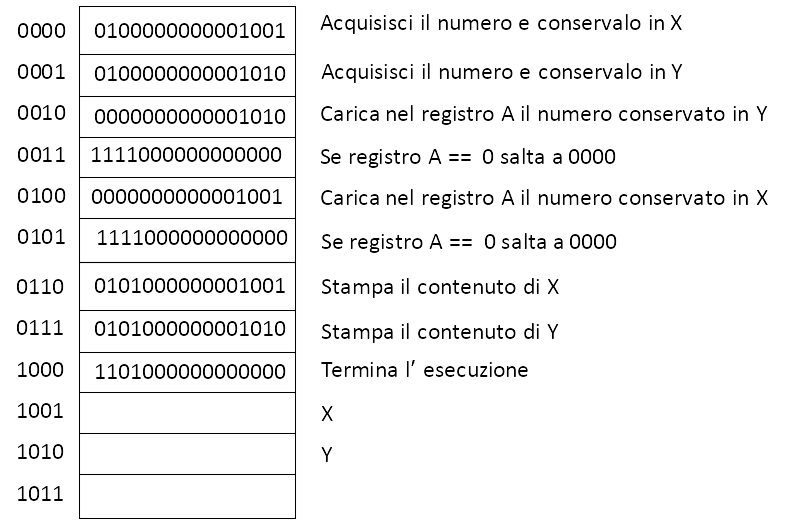
\includegraphics[width=0.6\linewidth]{./codice_macchina}
\pause

Si risponda alle seguenti domande:
\begin{enumerate}
\item Si descriva il comportamento dell'unità di elaborazione durante l'esecuzione dell'istruzione che si trova nella cella di indirizzo 0101.
\item Si costruisca lo schema a blocchi (anche chiamato diagramma di flusso) corrispondente al programma riportato sopra.
\item Si scriva un programma in linguaggio C che sia equivalente a quello dato.
\end{enumerate}
\end{frame}

\begin{frame}
\frametitle{Esercizio 7 - Soluzione 1}
All'inizio dell'esecuzione dell'istruzione, il PC contiene il valore 0101.

Nella fase di fetch l'unità di elaborazione acquisisce dalla memoria l'istruzione che si trova in questa cella di memoria e la copia nel Current Instruction Register (CIR). Il PC assume valore 0110.

Nella fase di interpretazione l'unità di controllo riconosce l'istruzione.

Nella fase di esecuzione l'unità di elaborazione verifica se il valore contenuto nel registro A è pari a 0. In caso affermativo, il valore del PC viene posto al valore dell'operando dell'istruzione e diventa quindi pari a 0000. 
\end{frame}

\begin{frame}
\frametitle{Esercizio 7 - Soluzione 2}
\centering
\makebox[\textwidth]{\resizebox{.8\linewidth}{!}{
		\begin{tikzpicture}[auto]
		\node [startstop] (start) {Inizio};
		\node [input, below = of start] (i0000) {Leggi X};
		\node [input, below = of i0000] (i0001) {Leggi Y};
		\node [block, below = of i0001] (i0010) {regA = Y};
		\node [decision, below = of i0010] (i0011) {regA == 0};
		\node [block, right = of i0011] (i0100) {regA = X};
		\node [decision, below = of i0100] (i0111) {regA == 0};
		\node [output, right = of i0111] (i1000) {Stampa X, Y};
		\node [startstop, below = of i1000] (stop) {Fine};
		
		\path [line] (start) -- (i0000);
		\path [line] (i0000) -- (i0001);
		\path [line] (i0001) -- (i0010);
		\path [line] (i0010) -- (i0011);
		
		\path [line] (i0011) -- +(-2,0) |- (i0000) node [near start] {true};
		\path [line] (i0011) -- (i0100) node [near start] {false};
		
		\path [line] (i0100) -- (i0111);
		\path [line] (i0111) -- +(-7,0) |- (i0000) node [near start] {true};
		\path [line] (i0111) -- (i1000) node [near start] {false};
		\path [line] (i1000) -- (stop);
		\end{tikzpicture}
	}}
\end{frame}

\begin{frame}
\frametitle{Esercizio 8 - Moltiplicazione per somme ripetute con numeri negativi}
Scrivere lo pseudocodice per eseguire la moltiplicazione di numeri negativi tramite somme ripetute.
\end{frame}


\begin{frame}
\frametitle{Esercizio 8 - Ricerca per bisezione}
\begin{enumerate}
	\item Leggi $op1$ e $op2$
	\item Se $abs(op1) \leq abs(op2)$:
	\begin{enumerate}
		\item $num=abs(op2), min=abs(op1)$
		\item Altrimenti: $num=abs(op1), min=abs(op2)$
	\end{enumerate}
	
	\item Se $(op1 < 0 \wedge op2 \geq 0) \vee (op1 \geq 0 \wedge op2 < 0)$:
	\begin{enumerate}%
		\item $num = -num$
	\end{enumerate}

	\item $ris = 0$
	\item Ripeti finché $min > 0$:
	\begin{enumerate}
		\item $ris = ris + num$
		\item $min = min - 1$
	\end{enumerate}
	\item Stampa $ris$ e termina
\end{enumerate}
\end{frame}

\begin{frame}
\frametitle{Esercizio 9 - Ricerca in sequenza ordinata}
Scrivere lo pseudocodice per cercare un valore all'interno di una sequenza, sfruttando il fatto che la sequenza è ordinata.
\end{frame}

\begin{frame}{Esercizio 9 - Soluzione in pseudocodice}
\begin{enumerate}
	\item Ricevo una sequenza \emph{s} di lunghezza \emph{l} e l'elemento cercato $c$
	\item Se $l == 1$ controllo l'unico elemento della lista $e$:
	\begin{enumerate}
		\item Se $e==c$ allora ho trovato $c$ e termino
		\item Se $e\neq c$ allora $c$ non esiste in $s$ e termino
	\end{enumerate}
	\item Altrimenti:
	\begin{enumerate}
		\item Considero l'elemento \emph{e} a metà di \emph{s}
		\item Se $e > c$ vado ad 1 utilizzando la prima metà di $s$ come nuova sequenza
		\item Altrimenti torno ad 1 utilizzando la seconda metà di $s$ (incluso $e$) come nuova sequenza
	\end{enumerate}
\end{enumerate}
Posso aggiungere una condizione 3.4 che controlla direttamente se $e == c$.
Se la stringa è di lunghezza pari posso prendere l'elemento immediatamente successivo (o precedente) alla metà esatta.
\end{frame}

\begin{frame}{Introduzione al C}
Risolvere in C i precedenti esercizi.
\end{frame}


\end{document}
